\documentclass[11pt,a4paper]{article}
\usepackage[T1]{fontenc}
\usepackage[utf8]{inputenc}
\usepackage[margin=2cm,includefoot,footskip=30pt]{geometry}
\usepackage{amsmath}
\usepackage{amssymb}
\usepackage{helvet}
\usepackage{graphicx}
\usepackage[dvipsnames]{xcolor}
\usepackage{pgfgantt}
\usepackage{parskip}
\usepackage[hidelinks]{hyperref}
\usepackage[polish]{babel}
\usepackage{float}

\renewcommand{\familydefault}{\sfdefault}
\renewcommand{\arraystretch}{1.5}

\begin{document}

    \begin{titlepage}
        \centering
        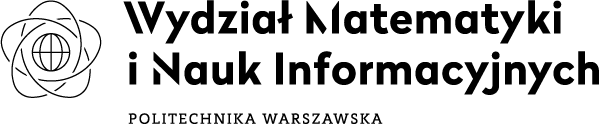
\includegraphics[width=\textwidth]{resources/WMiNI-znak-black.png} \par
        \vspace{3cm}
        {\LARGE Programy działań z efektami domyślnymi \par}
        \vspace{0.5cm}
        {\Large Reprezentacja Wiedzy - projekt \par}
        \vspace{2cm}
        {\large
            Bartosz Borkowicz\\
            Sebastian Konowrocki\\
            Tomasz Laskowski\\
            Piotr Łazarczyk\\
            Jakub Niemyjski\\
            Bartłomiej Pieńkowski\\
            Igor Pieńkowski\\
            Bartłomiej Teodorczuk\\
            Łukasz Wasilewski
        \par}
        \vspace{4cm}
        {\large Wersja 1.0 \par}
        \vspace{0.5cm}
        {\large \today \par}
    \end{titlepage}

    \tableofcontents
    \newpage

    \section{Opis zadania}
    
    Celem projektu jest opracowanie języka akcji oraz odpowiadającego mu języka kwerend dla klasy systemów dynamicznych, która została zdefiniowana poniżej.
    
    Język akcji ma być zaprojektowany dla klasy systemów dynamicznych spełniających następujące warunki:
    \begin{enumerate}
        \item Prawo inercji
        \item Niedeterminizm i sekwencyjność działań
        \item Pełna informacja o wszystkich akcjach i wszystkich skutkach bezpośrednich
        \item Z każdą akcją związany jest
            \begin{itemize}
                \item warunek początkowy (ew. $true$)
                \item efekt akcji
                \item jej wykonawca
            \end{itemize}
        \item Skutki akcji:
            \begin{itemize}
                \item \textit{pewne} - zawsze występują po zakończeniu akcji
                \item \textit{domyślne} - preferowane, zachodzą po zakończeniu akcji, o ile nie jest wiadomym, że nie występują
            \end{itemize}
        \item Efekty akcji zależą od stanu, w którym akcja się zaczyna oraz od jej wykonawcy
        \item W pewnych stanach akcje mogą być niewykonalne przez pewnych (wszystkich) wykonawców
    \end{enumerate}
    
    Język akcji spełniający dane warunki może być odpytywany poprzez odpowiadający mu język kwerend, który zapewnia uzyskanie odpowiedzi prawda ($true$) bądź fałsz ($false$) na następujące pytania:
    \begin{enumerate}
        \item Czy podany program działań jest wykonywalny zawsze/kiedykolwiek?
        \item Czy wykonanie podanego programu działań z dowolnego stanu spełniającego warunek $\pi$ prowadzi zawsze/kiedykolwiek/na ogół do stanu spełniającego warunek celu $\gamma$?
        \item Czy z dowolnego stanu spełniającego warunek $\pi$ cel $\gamma$ jest osiągany zawsze/kiedykolwiek/na ogół?
        \item Czy wskazany wykonawca jest zaangażowany w realizację programu zawsze/kiedykolwiek?
    \end{enumerate}

    \section{Język akcji}
    
    \subsection{Sygnatura}
    
    \subsection{Syntaktyka}
    
    \subsection{Semantyka}
    
    \section{Język kwerend}
    
    \subsection{Syntaktyka}
    
    \subsection{Semantyka}
    
    \section{Przykłady}
    
\end{document}